\documentclass[a4paper]{article}

\usepackage[english]{babel}
\usepackage[utf8x]{inputenc}
\usepackage{amsmath}
\usepackage{amsfonts}
\usepackage{graphicx}
\usepackage[]{algorithm2e}
\usepackage[colorinlistoftodos]{todonotes}

\title{CS 5785 -- Applied Machine Learning -- Lec.\ 12}
\author{Prof.\ Nathan Kallus, \\Scribe:Anastasios Belesiotis, Saniya Shah, Yingying Zheng}
\date{Oct.\ 4, 2018}

\begin{document}
\maketitle

\section{Principal Components Analysis (PCA)}
PCA is an unsupervised dimensionality reduction technique used to find axes of variations in a dataset.  In a sense, clustering may also be viewed as an unsupervised dimensionality reduction technique, in that it assigns possibly high dimensional feature vectors to one of $K$ tokens (cluster labels). Clustering is useful when the data is \textit{clumpy}, e.g., arranged in a manner reminiscent of Gaussian point clouds. For example, if a group of people play darts on a single target the darts would be arranged in a clump around the bullseye. Clumpy data is well represented by tokens or cluster centers. PCA is useful for ``manifoldy'' data (specifically, linear manifolds), which is well represented in low dimension coordinate system.  Often, problems that are well suited to $K$-means are ill suited to PCA and vice versa.

\begin{figure}
\centering
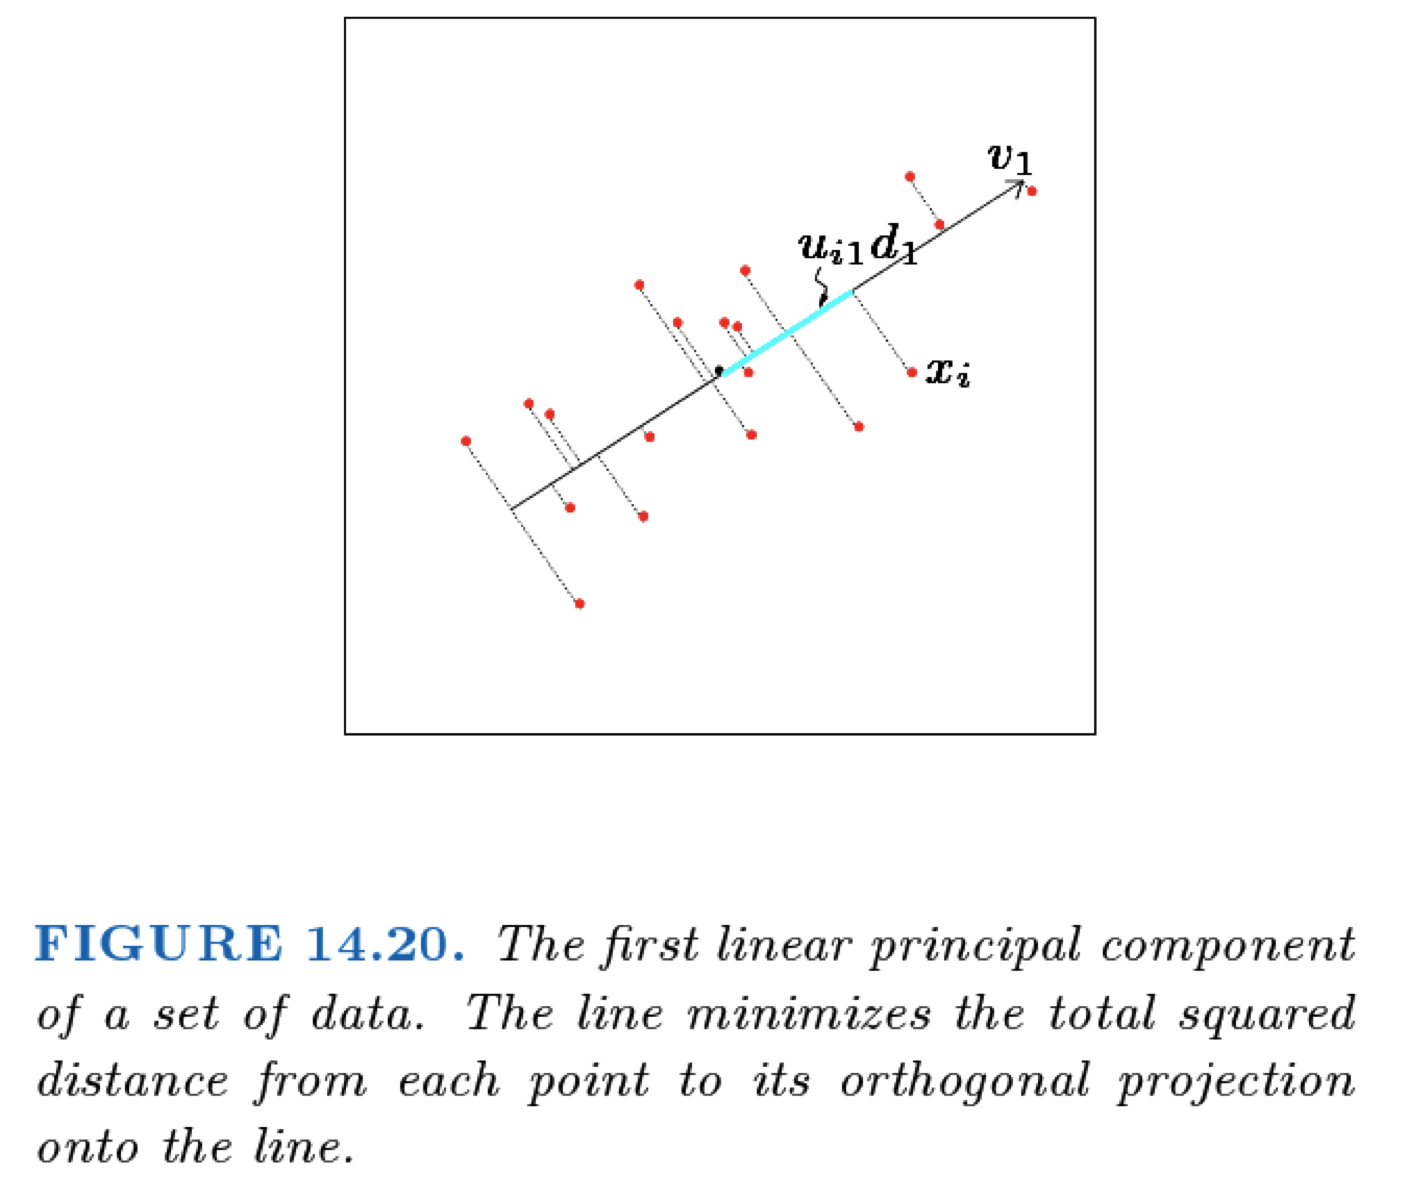
\includegraphics[width=1.0\textwidth]{TwoDimReduction.png}
\caption{\label{fig:2DimReduction} }
\end{figure}

As a simple example of dimensionality reduction, suppose you collect the feet length and width measurements for a group of people.  This yields a list of 2D feature vectors per person.  We would like to ``project this down'' to 1D in a manner that captures as much of the variability in the data ase possible.  In particular, if we can find the axis with greatest variance
as shown in Figure \ref{fig:2DimReduction}, the single coordinate of each data point along that axis could be a good choice for a reduced dimensionality representation of the data.

PCA attempts to capture the axes of variation by a sequence of projections of a dataset, mutually uncorrelated and ordered in variance. Being mutually uncorrelated we get a set of projections that do not contain duplication of data and assure we have the minimal set of projections containing the amount of data we need. By ordering the projections in variance we gain the ability to drop projections at the end of the list that are uninformative, that can perhaps be considered as noise, and by doing so reduce the dimentionality.\\

Given a set of $N$ points $x_i \in \mathbf{R}^p$, we suppose that they live on a linear manifold, rather than simply filing up $\mathbb{R}^p$ in an unstructured manner. The idea behind dimensionality reduction that PCA attempts to solve is to keep the best \emph{rank $q$ approximation} of the data for some $q<p$.  The model for representing the data is a non-parametric representation of an affine hyperplane of rank $q$:
$$f(\lambda)= \mu+\mathbf{V}_q \lambda$$
Where:
\begin{itemize}
\item $\mu$: a location vector in $\mathbf{R}^p$, can also be viewed as the ``centered'' origin of the data.
\item $\mathbf{V}_q \in \mathbf{R}^{p\times q}$, with $q$ orthogonal unit vectors as its columns.
\item $\lambda$: a vector of $q$ parameters.
\end{itemize}

\begin{figure}
\centering
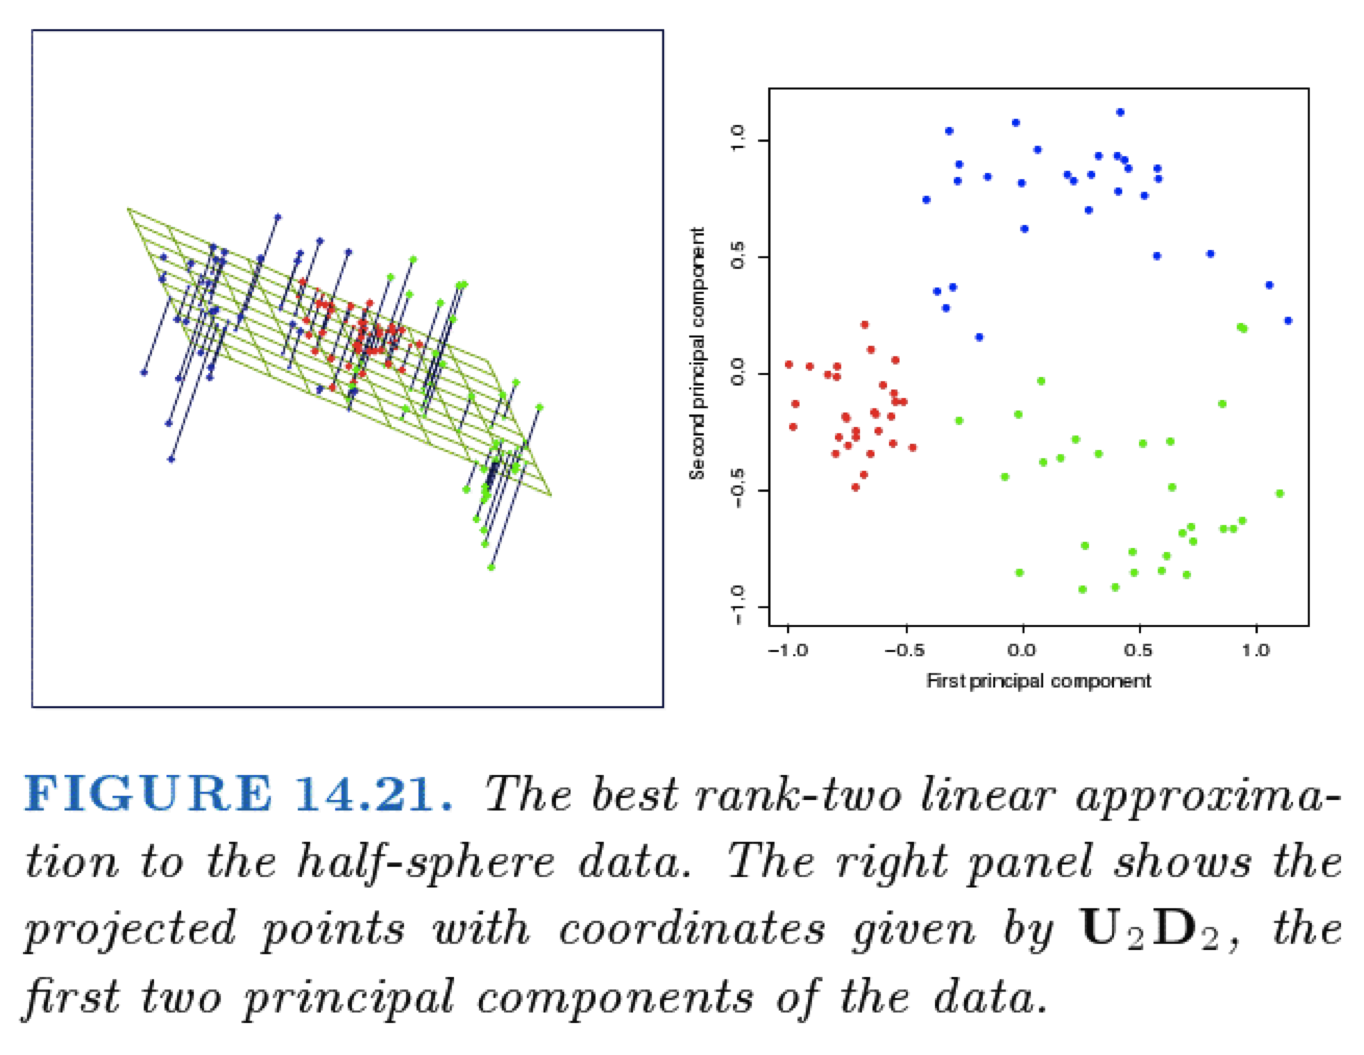
\includegraphics[width=1.0\textwidth]{ThreeDimReduction.png}
\caption{\label{fig:3DimReduction}}
\end{figure}

Figure \ref{fig:2DimReduction} is an example of a dimensionality reduction where $p=2$ and $q=1$. In Figure \ref{fig:3DimReduction} $p=3$ and $q=2$. 

We want to find the matrix $\mathbf{V}_q$ and vector $\lambda$ that generate the smallest reconstruction error. This is a least squares fitting problem:
$$\min_{\substack{
   \mu \\
   {\lambda_i} \\
   \mathbf{V}_q
  }} \sum_{i=1}^N \| x_i-\mu-\mathbf{V}_q\lambda_i \|^2$$
  
It is relatively straightforward to show that the optimal $\mu$ and $\lambda_i$s are given by:
\begin{itemize}
\item $\hat{\mu}=\bar{x}$: The new origin is the average of all the original data points, the center of the data.
\item $\hat{\lambda}_i=\mathbf{V}_q^\top(x_i-\bar{x})$: The projection after centering around the mean.
\end{itemize}

We are left with finding the optimal orthogonal matrix $\mathbf{V}_q$:
$$\min_{\mathbf{V}_q} \sum_{i=1}^N \| (x_i-\bar{x})-\mathbf{V}_q\mathbf{V}_q^\top(x_i-\bar{x})\|^2$$

For simplicity, assume we have a \textit{centered} set of data, i.e., $\bar{x}=0$, and we get:
$$\min_{\mathbf{V}_q} \sum_{i=1}^N \| x_i -\mathbf{V}_q\mathbf{V}_q^\top x_i \|^2$$
Where $\mathbf{V}_q\mathbf{V}_q^\top$ is a $p\times p$ projection matrix. Denote $\mathbf{M}_q=\mathbf{V}_q\mathbf{V}_q^\top$. $\mathbf{M}_q$ maps each $x_i$ onto its rank $q$ reconstruction, the orthogonal projection of $x_i$ onto the subspace spanned by the columns of $\mathbf{V}_q$. If $ p = q $, $\mathbf{V}_q\mathbf{V}_q^\top$  is an identity matrix.

We've already seen the machinery we need to solve this for $\mathbf{V}_q$: the SVD of $\mathbf{X}$, where $\mathbf{X}$ is formed by stacking the (centered) observations into the rows of an $N\times p$ matrix. The SVD of $\mathbf{X}$ is $\mathbf{U}\mathbf{D}\mathbf{V}^\top$, where $\mathbf{D}$ is a diagonal matrix with values $d_1, \ldots, d_p$ where: $d_1 \geq \ldots \geq d_p \geq 0$.
For each rank $q$ the solution to $\mathbf{V}_q$ above is given by the leading $q$ singular vectors in $\mathbf{V}$ (from the SVD). The columns of $\mathbf{UD}$ are the principal components of $\mathbf{X}$. The projection onto the sungular vectors gives us coordinates in a linear subspace, as shown in the right graph in Figure \ref{fig:3DimReduction}.

The sample covariance for $\mathbf{X}$, assuming it is centered, is:
$$\mathbf{S}=\frac{1}{N}\mathbf{X}^\top\mathbf{X}\in\mathbb{R}^{p\times p}$$
PCA computes the eigenvectors of $\mathbf{S}$ to reveal the orthogonal axes of variation in the data that capture the most variance, meaning the axes where the data spreads the most. PCA does this by throwing away small eigenvalues and their corresponding eigenvectors to leave the highest $q$ singular values.

\end{document}